\chapter{Hybrid Eulerian-Lagrangian Vortex Particle Method}
\label{ch:hybrid}
%\label{ch:LiteratureReview}

%\section{Theory of Domain Decomposition Method}
% Comparison of hybrid vortex methods.
% choice of hybrid method. Example domain decomposion, coupling technique
%\subsection{Advantage of domain decomposition}

%%\subsection{Assumptions and Limitations}

%\subsection{Modified coupling strategy}
%\section{Theory}
%% What is hybrid vortex method?
%% What is the general idea behind the hybrid vortex method?
%% What does it mean to couple particle solver and grid solver?
%% What is the advantage?
%% What is the drawback?




\section{Eulerian-Lagrangian coupling algorithm}


	
%	\begin{figure}[h]
%	\centering
%	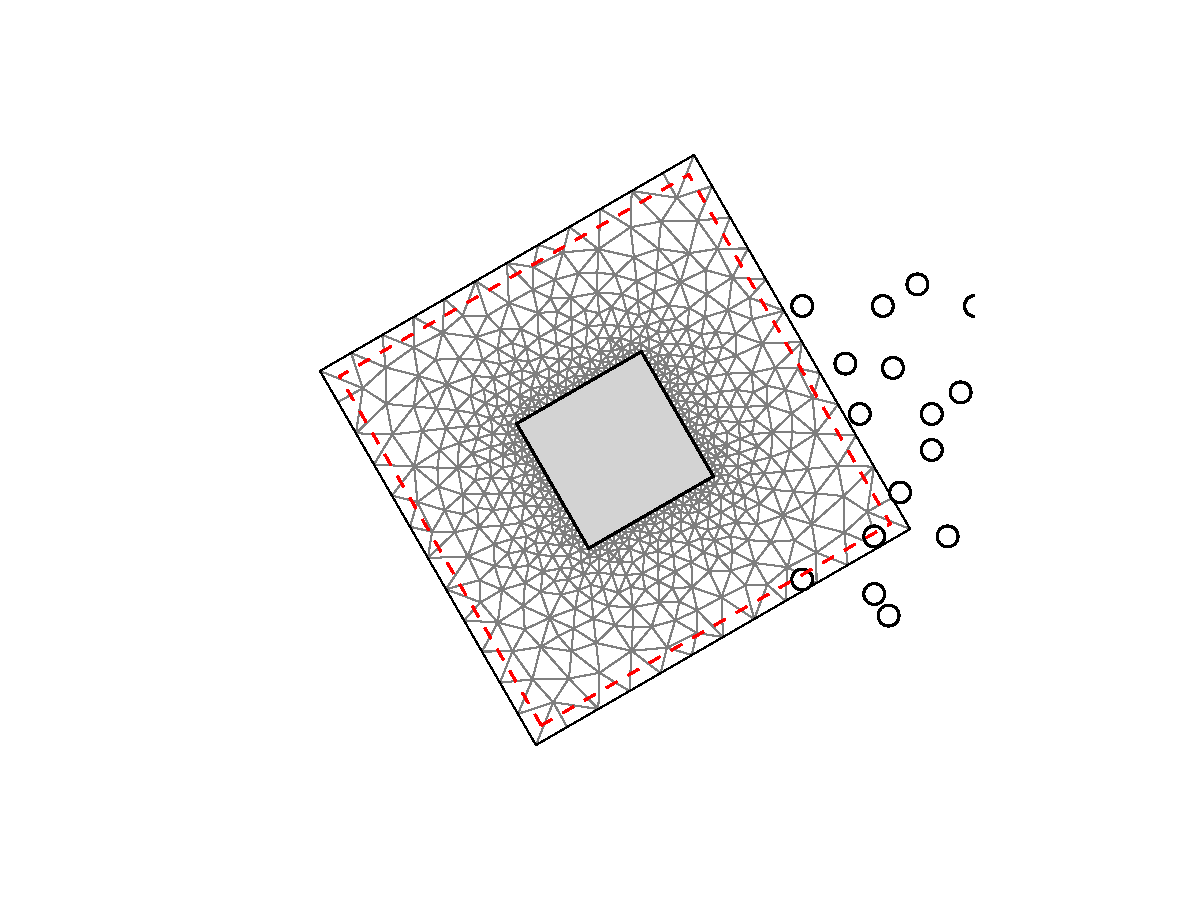
\includegraphics[trim=4.37cm 1.58cm 3.86cm 1.58cm, clip, width=0.5\linewidth]{./figures/hybrid/interpolation/particleRemoved.pdf}
%	\caption{interpolation FE2StructuredGrid withData}
%	\label{fig:testFig}
%	\end{figure}	
	
%	\begin{figure}[h]
%	\centering
%	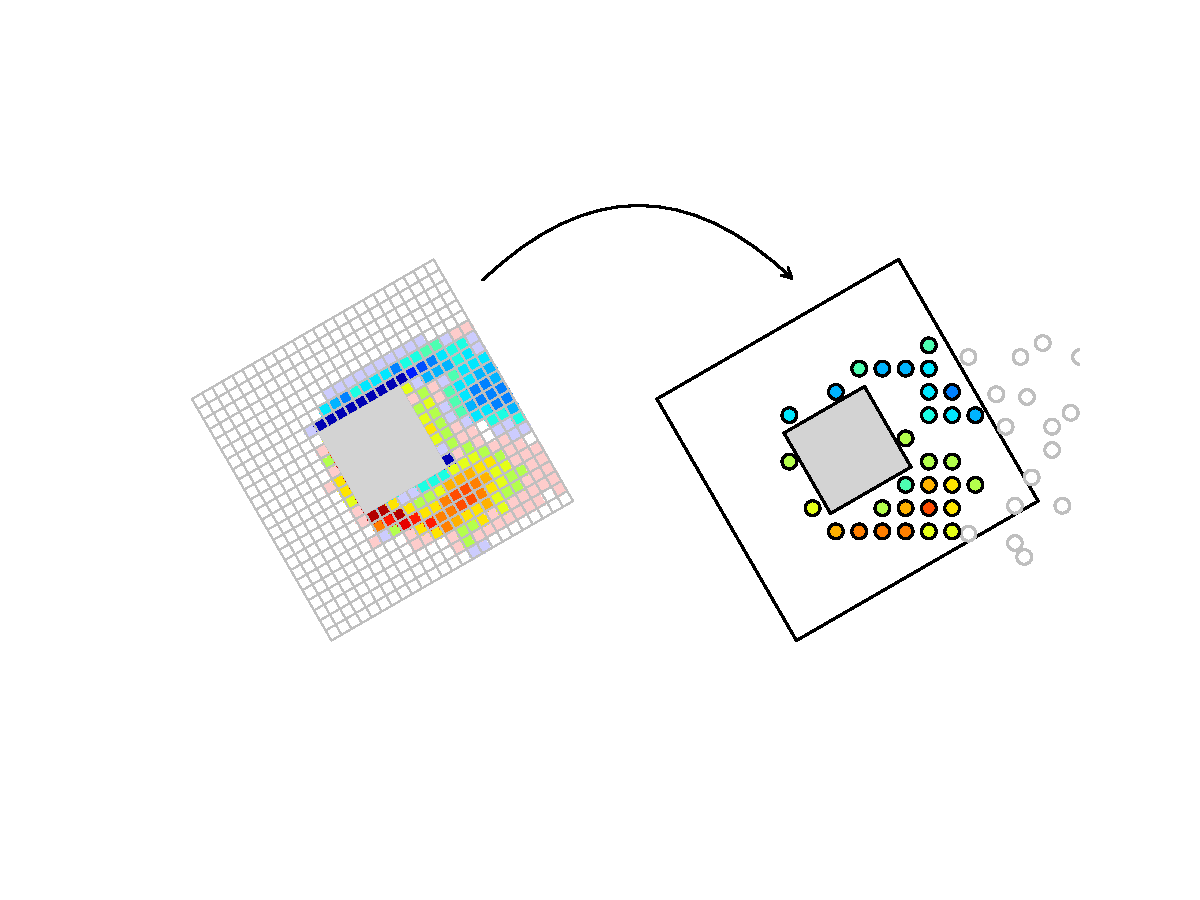
\includegraphics[trim=2.55cm 3.35cm 2.05cm 3.35cm, clip, width=\linewidth]{./figures/hybrid/interpolation/interpolation_StructuredGrid2Blobs.pdf}
%	\caption{interpolation FE2StructuredGrid withData}
%	\label{fig:testFig}
%	\end{figure}		
	
	\begin{figure}[t]
	\centering
	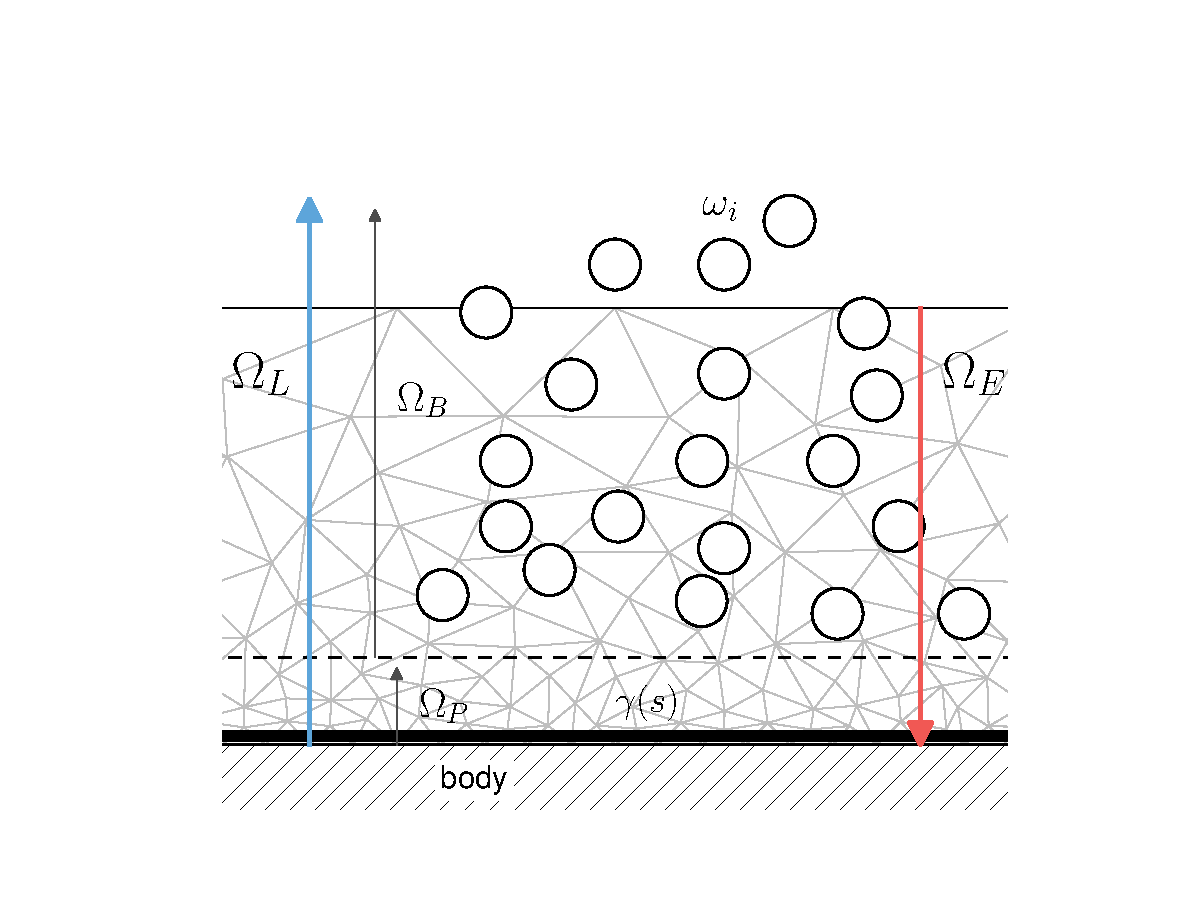
\includegraphics[width=0.7\linewidth]{./figures/hybrid/interpolation/hybrid_domains.pdf}
	\caption{hybrid domains}
	\label{fig:hybrid_domains}
	\end{figure}


\subsection{Eulerian dirichlet boundary condition}

	
	\begin{figure}[t]
	\centering
	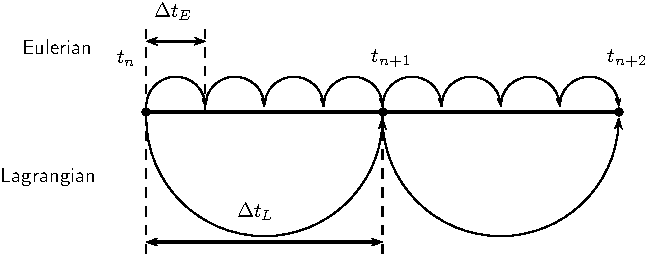
\includegraphics[width=0.7\linewidth]{./figures/eulerian/multiStep-crop.pdf}
	\caption{Eulerian multi-stepping to match the lagrangian $\Delta t_L$. The figures shows $\Delta t_L = 4 \Delta t_E$ and required $k_E = 4$ iterations to time march from $t_n$ to $t_{n+1}$.}
	\label{fig:multiStep}
	\end{figure}	


When coupling with the Lagrangian method, we will see that $\Delta t_E \leqslant \Delta t_L$ (Lagrangian time step size is ideally larger than Eulerian time step size), meaning that we will have to perform $k_E$ Eulerian sub-steps to reach the Lagrangian step, figure \ref{fig:multiStep}.

\subsection{Vorticity interpolation algorithm}

\section{Introduction to pHyFlow: Hybrid solver}

\subsection{Program structure}

\section{Summary}



%
%\section{Particle-Grid Coupling techniques}
%% Multiple ways of coupling , VIC, domain decomposition technique
%\subsection{Vortex in Cell method}
%
%\subsection{Particle-Grid domain decomposition methods}
%
%\section{Vortex diffusion methods}
%
%\subsection{Random walk method}
%\subsection{Core expansion method}
%\subsection{Particle-Strength Exchange}
%\subsection{Modified interpolation kernel for diffusion}
%
%\section{Simulation acceleration techniques}
%
%\subsection{Fast multi-pole Method}
%
%\subsection{Parallel computation in GPU}

%\section{Former Work}
%\label{sec:FormerWork}
%
%\subsection{Overview of the Work}
%\label{subsec:OverviewoftheWork}

%\section{Purpose of further research}

%%%%%%%%%%%%%%%%%%%%%%%%%%%%%%%%%%%%%%%%%%%%%%%%%%%%%%%%%%%%%%%%%%%%
%\nomenclature[ak]{$K$}{Kelvin (temperature)}
%\nomenclature[ar]{rpm}{Revolutions per minute (frequency)}
%\nomenclature[ac]{CO}{Carbon Monoxide}
%\nomenclature[ac]{CRM}{Chemical Reaction Modelling}
%\nomenclature[ah]{H2}{Molecular hydrogen}
%\nomenclature[ag]{GSP}{Gas Turbine Simulation Program (Software)}
%\nomenclature[rr]{$\rho$}{Density \nomunit{[$kg/{m^3}$]}}
%\nomenclature[sm]{$\dot{m}$}{Mass flow rate \nomunit{[$kg/s$]}}
%\nomenclature[ab]{bar}{Pressure}

%\nomenclature[rr]{$Re$}{Reynolds number \nomunit{[-]}}
%\nomenclature[rw]{$M$}{Mach number \nomunit{[-]}}
%\nomenclature[rw]{$\mu$}{Dynamic viscosity of air \nomunit{[$kg/{s \cdot m}$]}}